\documentclass{pgnotes}

\title{Advanced cooling}

\begin{document}

\maketitle

\section{Airflow}

\autoimage{cooling_airflow}{Airflow from Downflow CRAC through raised floor}{cooling-airflow}
\begin{itemize}
\item Warm \textbf{return air} enters the CRAC via an opening on the top of the unit.
  Sometimes the return air is ducted to the unit from above the ceiling.
\item Cold \textbf{supply air} leaves the CRAC via an opening in the bottom:
  \begin{itemize}
  \item If there is a raised floor, the cold air is blown out the bottom of the unit under the raised floor.
    It flows under the raised floor and exits through perforated tiles.
  \item In the case of a solid floor, the cold air normally leaves via a large grille on the bottom of the unit.
  \end{itemize}
\end{itemize}
Other configurations include upflow (reverse of the above, but only on a solid floor), horizontal and other configurations.
Cooling units are sometimes located in other areas and ducted to the data centre environment.

For the cooling system to work properly, we \textbf{must use a hot aisle / cold aisle arrangement}.
Where a raised floor is used, the perforated tiles must be in the cold aisle, and not in the hot aisle.

\section{DX units}

We have already met the self-contained air cooled DX and the standard split DX CRAC.

\newpage
\subsection{Glycol-cooled DX}

The Glycol-cooled DX replaces the air-cooled condenser with a refrigerant-to-fluid condenser inside the CRAC casing, \autoref{fig:crac-dx-glycol-dry-cooler}.
Liquid coolant consisting of water mixed with ethylene glycol is circulated between the condenser and a \textit{dry cooler} (coil with a fan) by a \textit{pump package}.

\begin{figure*}[hptb]
  \centering
  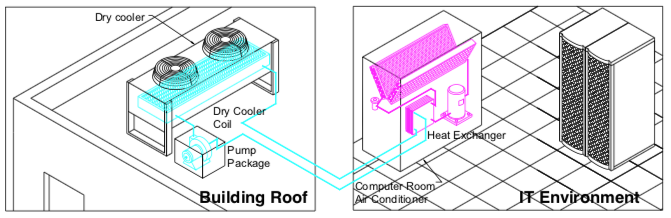
\includegraphics[width=1.0\linewidth]{crac_dx_glycol_schematic}
  \caption{DX Glycol-cooled CRAC with Dry Cooler (APC)}
  \label{fig:crac-dx-glycol-dry-cooler}
\end{figure*}

A dry cooler (as distinct from a wet cooler aka cooling tower (see later)) visually looks the same as a condenser, \autoref{fig:dry-cooler-photo}.

\begin{figure}[htbp]
    \centering
    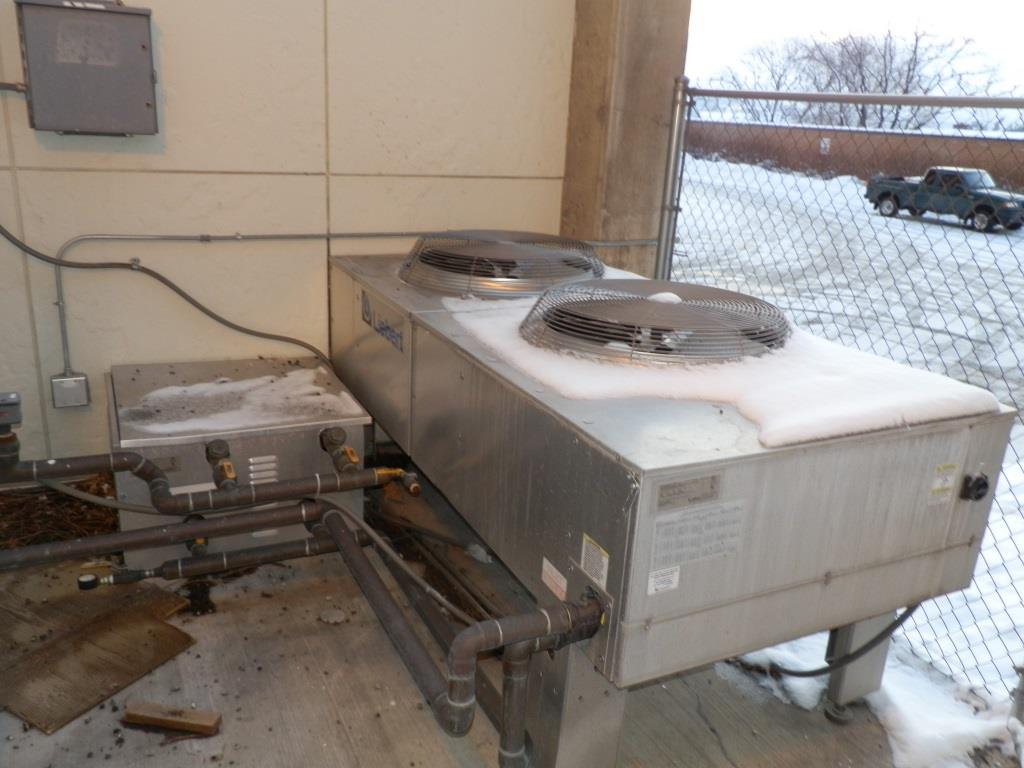
\includegraphics[width=0.4\linewidth]{dry_cooler_photo}
    \caption{Dry cooler photo}
    \label{fig:dry-cooler-photo}
\end{figure}

Some advantages of this system are:
\begin{itemize}
\item Refrigeration circuit is sealed inside the CRAC.
\item Glycol can be pumped much longer distances.
\item Can bypass the refrigeration system if the ambient air is cool enough. Glycol pumped through an economizer coil instead. See later on!
\end{itemize}

Candidate for \SIrange{30}{1000}{\kilo\watt}, and over longer distances.
Systems can either be:
\begin{description}
\item[Unitary] where a single CRAC is linked to a single dry cooler.
\item[Shared] where a number of CRACs share one or more dry coolers.
\end{description}

\newpage
\subsection{Water-cooled DX}

The Water-cooled DX is similar to the glycol-cooled version, except that a water loop is used instead of a glycol loop.

\begin{figure*}[hptb]
  \centering
  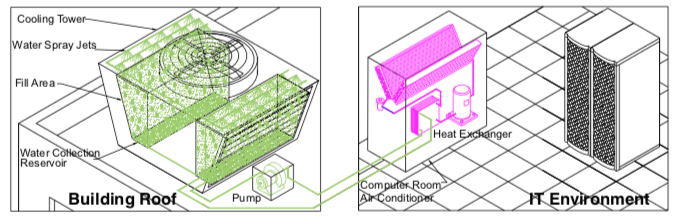
\includegraphics[width=1.0\linewidth]{crac_dx_water_schematic}
  \caption{DX water-cooled CRAC with cooling tower (APC)}
  \label{fig:crac-dx-water-schematic}
\end{figure*}

The dry cooler is replaced with a \textit{cooling tower} (or wet cooler, as distinct from a dry cooler), often on the facility's roof, where jets of water are cooled by spraying them into a moving air stream.

\begin{figure}[htbp]
    \centering
    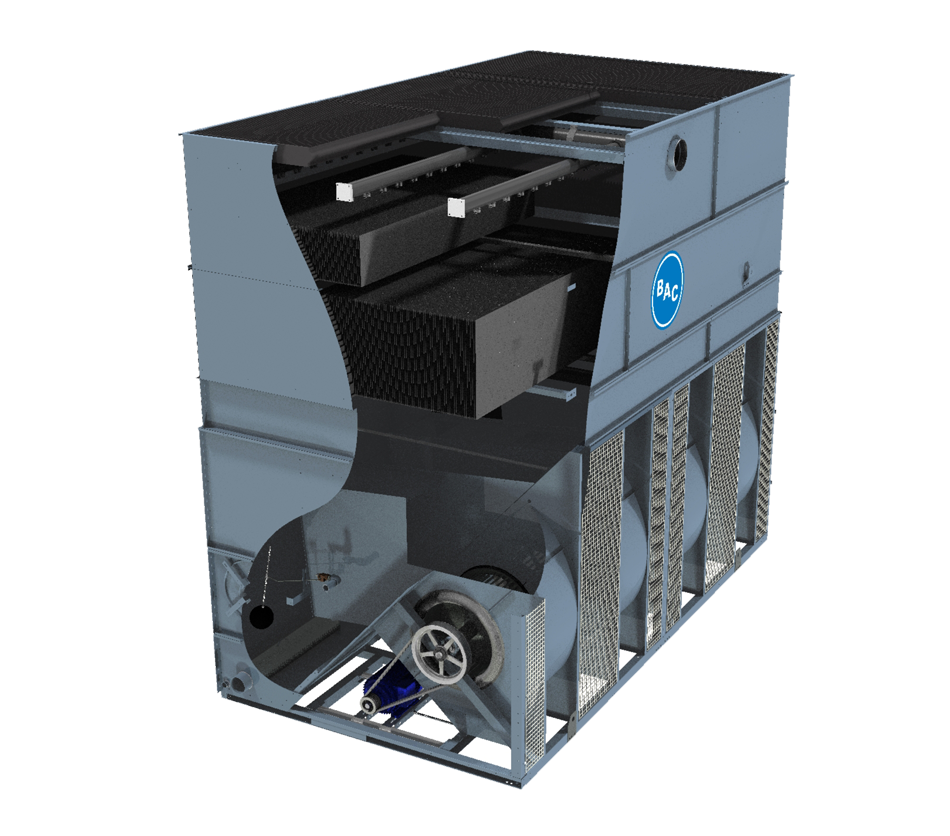
\includegraphics[width=0.4\linewidth]{cooling_tower_baltimore}
    \caption{Cooling tower (Baltimore)}
    \label{fig:cooling-tower-photo}
\end{figure}

It is more efficient that Glycol-based systems in hot dry climates, where evaporation in the cooling tower assists with its operation.
However, the water treatment must be carefully considered.
There is also a strong risk of legionella in these systems if not properly looked after.

Water cooled DX is rarely installed in a unitary fashion.
One or more shared cooling towers servicing multiple CRACs with cooled water is by far the most common configuration.

Cooling towers are sometimes operated by facilities management or by the landlord in larger buildings, and water is supplied metered or unmetered ``as a service''.
Very common in office blocks, shopping centres. 
The same towers often serve not only technical cooling, but also comfort cooling, process cooling and refrigerated storage (for food and other products) systems.

\section{Chilled water cooling systems}

Chilled water cooling systems involve the supply of chilled water to Computer Room Air Handlers (CRAH) in the data centre environment.
CRAHs are similar to CRACs in appearance, and are available in the same wide range of airflow configurations.
They are simpler than CRACs, containing only a blower fan, finned water coil and controls.

\begin{figure}[htbp]
  \centering
  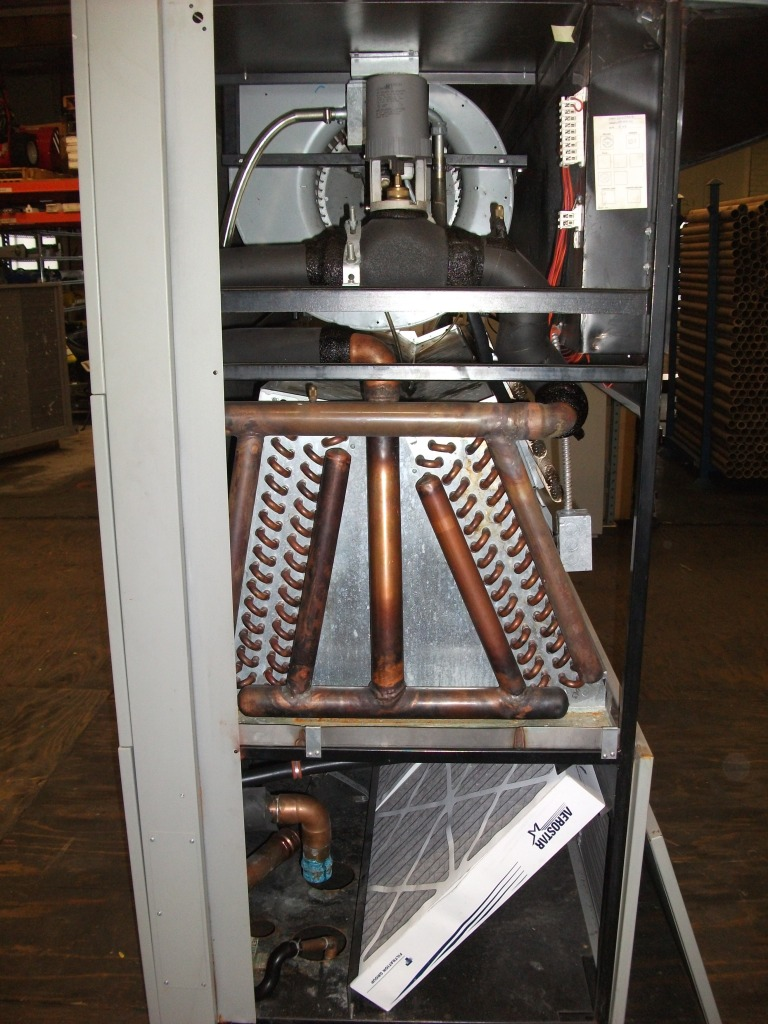
\includegraphics[width=0.3\linewidth]{crah_side_view}
  \caption{CRAH side view}
  \label{fig:crah-side-view}
\end{figure}

The chilled water is produced in a separate \textit{chiller}.
The chiller rejects heat from the chilled water loop to the atmosphere in similar ways to DX CRACs.
Air-cooled, glycol-cooled and water cooled chillers are all very common.

\begin{figure}[htbp]
  \centering
  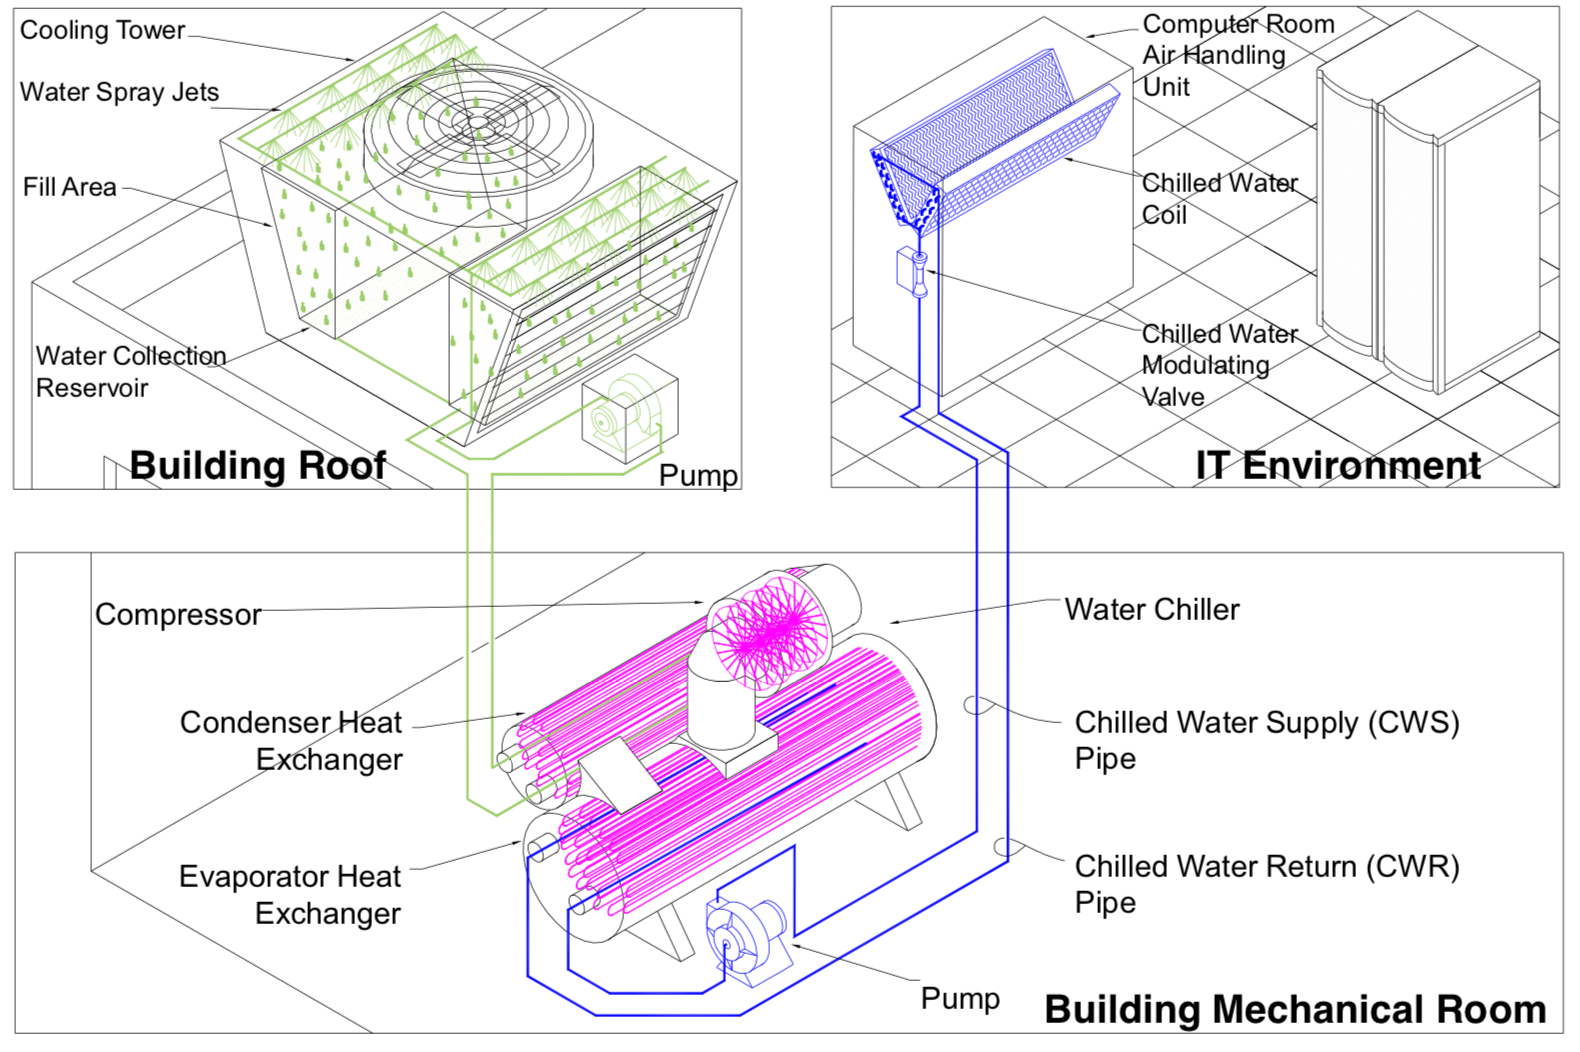
\includegraphics[width=1.0\linewidth]{chilled_water_system_water_cooled}
  \caption{Chilled water system}
  \label{fig:chilled-water-system-water-cooled}
\end{figure}

Although \autoref{fig:chilled-water-system-water-cooled} depicts a unitary system, chilled water systems are almost always installed such that a large number of CRACs or other cooling loads are served by a small number of chillers and cooling towers / fluid coolers.
Chilled water systems also can incorporate large buffer tanks for load balancing, energy price optimisation and to provide \textit{ride through} in case of power failure.

Many buildings, particularly city skyscrapers, use centralised water-cooled chilled water system. 
A small number of very large cooling towers serve a number of chillers which supply chilled water for data centre, comfort cooling and other cooling purposes.
These are generally managed by facilities personnel. 

In a multi-tenant building, the landlord will often supply chilled water as a metered chargeable service to tenants.
Condenser loop water is often also available at a much cheaper unit rate (which can be used for a DX water-cooled CRAC or local water-cooled chiller for IT purposes).

\end{document}

